\chapter{Předpoklady}
\label{requirements}

V úvodu jsme uvedli, že budeme pracovat s \textbf{Labeled-property} grafovým modelem a dotazy nad daným modelem budou provedeny v jazyku PGQL.
V této kapitole popíšeme konkrétněji daný model a jazyk.

\section{Labeled-property datový model}
\label{req.propGraph}

Při zpracování této práce uvažujeme grafovou databázi, která pracuje s grafovým modelem \textbf{Labeled-property}\footnote{\url{https://en.wikipedia.org/wiki/Graph_database} [dostupnost ověřena k datu 8.5.2021]}.
V této sekci popíšeme Property graf a jeho vlastnosti z pohledu grafové databáze.
Překvapivě neexistuje standartní definice daného modelu, ačkoliv je značně využíván v moderních systémech.
Proto budeme pracovat s popisem Property grafu systému Neo4j \citep{neopropertygraph} a definicí jazyka PGQL \citep{pgql}.
Na základě těchto popisů určíme klíčové vlastnosti Property grafu, které budeme uvažovat v naši práci.

\subsubsection{Obecný popis Property grafu}
Obecně grafová dazabáze pracující s daným modelem organizuje grafová data do tří částí:

\begin{itemize}
\item První část obsahuje množinu \textbf{vrcholů} (Vertices).
Vrcholy zde představují entity nebo doménové komponenty grafu.
Vrchol tedy reprezentuje objekt, osobu, myšlenku, dílo a podobně.

\item Druhá část obsahuje množinu \textbf{hran} (Edges).
Hrany jsou zde vždy orientované a spojují dva vrcholy.
Hrany zde představují vztahy mezi vrcholy.
Hrana tedy může být například vztah kamarádství dvou lidí (Karel \textit{se kamarádí s} Jirkou.), vztah zaměstnání člověka se zaměstnavatelem (Karel \textit{pracuje pro Google.}) a podobně.
Vrcholy a hrany zde označíme za \textbf{elementy} grafu.
\item Poslední třetí část představuje \textbf{vlastnosti} (Properties) a \textbf{štítky} (Labels), které jsou uloženy v elementech grafu.

\begin{itemize}
\item
Štítek představuje označení určité skupiny nebo chování.
Každému elementu může být přiděleno několik štítků.
Na elementy, kterým byl přidělen stejný štítek, se můžeme dívat jako na skupinu.

\item
Vlastnosti definují dvojice (\texttt{název, hodnota}).
První z dvojice \texttt{název} udává název vlastnosti a \texttt{hodnota} udává hodnotu dané vlastnosti.
Hodnota vlastnosti má také vždy definován svůj skalární \textbf{typ} (například číselná hodnota nebo řetězec).
Každému elementu může přináležet několik vlastností.
Avšak, jeden element nemůže mít dvě dvojice sdílející název.
Navíc pokud dva různé elementy sdílejí vlastnost (tj. mají stejný název), pak typy hodnoty vlastnosti musí být rovněž totožné.
\end{itemize}
\end{itemize}

\subsubsection{Omezení Property grafu}
Popsali jsme obecně Property graf.
Daný popis modelu je značně abstraktní, proto si určíme další zpřísňující vlastnosti, které budeme využívat v naši práci.

\begin{enumerate}

\item
Každý element bude mít unikátní identifikátor (\texttt{ID}), abychom dokázali rozlišovat dané elementy.
\texttt{ID} zde nechápeme jako vlastnost elementů, ale jako interní značení uvnitř grafu.

\item
Každý element (vrchol/hrana) bude mít právě jeden štítek.
Myslíme, že počet štítků není určující pro naši práci, protože primárně ovlivňuje prohledávání grafu a ne části \textit{Order by} nebo \textit{Group by}.

\item
Budeme uvažovat, že štítky vrcholů jsou vždy rozdílné od štítků hran.

\item
Každému štítku přiřadíme výčet vlastností.
To znamená, že štítek nemusí mít žádnou vlastnost nebo jich má určitý počet.

\item
Štítky mohou sdílet vlastnosti, ale vlastnosti musí mít stejný typ hodnoty.
To znamená, že i štítek hrany se štítkem vrcholu může mít stejnou vlastnost, pokud mají stejný typ hodnoty.

\end{enumerate}

Samotná grafová data nebudeme nijak omezovat.
To znamená, že v grafu mohou být cykly, dva vrcholy mohou být propojeny několika hranami, nemusí existovat žádná hrana ani vrchol, mohou existovat nepropojené vrcholy, hrana může mít totožný počáteční vrchol s koncovým vrcholem a podobně.

\subsubsection{Příklad grafu splňující model}
Nyní uvedeme příklad jednoduchého grafu splňující náš model:

\begin{figure}[!htp]
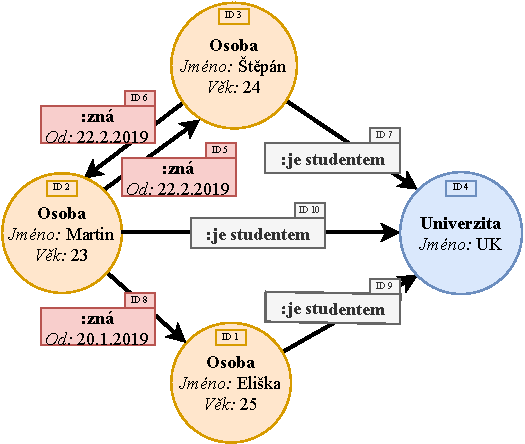
\includegraphics[width=100mm]{../img/propertyexample.pdf}\centering
\caption{Příklad Property grafu.}
\label{figure.propertygraphexample}
\end{figure}

Na obrázku \ref{figure.propertygraphexample} vidímě tři vrcholy se štítkem \textbf{Osoba}, které reprezentující fyzické osoby, a jeden vrchol se šítkem \textbf{Univerzita} reprezentující vysokou školu.
Štítku \textbf{Osoba} byly přiděleny dvě vlastnosti: \textit{Jméno} (řetězec) a \textbf{Věk} (číselná hodnota).
Štítku \textbf{Univerzita} byla přidělena jedna vlastnost: \textit{Jméno}, která odpovídá stejné vlastnosti štítku \textbf{Osoba} a mají stejný typ hodnoty (řetězec).
Mezi vrcholy fyzických osob existuje vztah \textbf{zná}, který určuje zda jedna osoba (počáteční vrchol) zná druhou osobu (koncový vrchol).
Vlastnost \textit{Od} definuje datum, kdy došlo k poznání osoby.
Mezi vrcholy fyzických osob a vysokou školou existuje vztah \textbf{je studentem}, který říká zda osoba studuje na dané vysoké škole.
Tento vztah nemá žádnou vlastnost.
Samotně pak každý element má přiřazeno \texttt{ID}.
Příklad vznikl na základě prvního grafu z dokumentace níže popisovaného PGQL.

V průběhu práce budeme graf splňující daný model označovat jako \textbf{Property graf}.

\section{Jazyk PGQL}
\label{req.pgql}

V naši práci budeme používat dotazovací jazyk PGQL \citep{pgql} verze 1.2 k dotazování nad Property grafem.
Jazyk je značné obsáhlý a k realizaci naši práce nepořebujeme všechny jeho vlastnosti, proto jsme se rozhodli využít jeho podmnožinu.
V naši práci budeme pracovat jen s částmi \textit{Select}, \textit{Match}, \textit{Group by} a \textit{Order by}.
Ostatní části nebudeme používat.
V každém dotazu musí být vždy přítomná část \textit{Select} a \textit{Match}.
S části \textit{Match} se pojí část \textit{From} specifikující název grafu, nad kterým se má vykonat dotaz.
Nicméně, v naši práci vždy budeme pracovat s jedním grafem a tedy jsme část vyřadili. 
Zároveň v naši práci uvažujeme, že \textit{Order by} a \textit{Group by} nejsou zadány nikdy společně.

\begin{itemize}
\item \textit{Match:} definuje podgraf, který bude vyhledán v grafu.
Součástí definice podgrafu jsou proměnné, které jsou přístupné v ostatních částech dotazu.
Proměnná zde reprezentuje jeden element podgrafu.

\item \textit{Select:} určuje vrácená data ve formě tabulky jako u tabulkových databazí.
K jednomu výsledku tak můžeme vrátit výčet informací.
Každá položka výčtu pak definuje jeden sloupeček tabulky.

\item \textit{Group by:} dovoluje seskupit výsledky dle zadaných klíčů a vypočítat agregační funkce pro výsledné skupiny.

\item \textit{Order by:} vykoná setřídění výsledků dle zadaných klíčů.
\end{itemize}

Nyní krátce popíšeme omezení a klíčové vlastnosti, s kterými budeme pracovat.
Pro komplexní popis odkazujeme na citovanou dokumentaci.

\subsubsection{Match}

Část \textit{Match} se skládá z posloupností elementů definující hledaný podgraf.
Posloupnosti jsou odděleny čárkou.
Položky v posloupnosti jsou vrcholy a hrany.
Položky vrcholů značíme pomocí \texttt{()} a položky hran pomocí šipek \texttt{->} (dopředná hrana), \texttt{<-} (zpětná hrana) a \texttt{-} (libovólná hrana).

Každé položce je možno přidělit jméno (definice proměnné) a predikát štítku.
Vrcholu přidělíme proměnnou vložením jména do kulatých závorek: \texttt{(jméno)}.
Hraně přidělíme proměnnou vložením jména do hranatých závorek: \texttt{-[jméno]->}, \texttt{<-[jméno]-} a \texttt{-[jméno]-}.
V části \textit{Match} musí být vždy přítomna alespoň jedna proměnná.
Pokud se v posloupnostech opakují proměnné zmená to, že v průběhu hledání musí dané položky obsahovat elementy se shodným \texttt{ID}.
Nicméně, proměnné hran se nesmí opakovat.
Pokud dvě posloupnosti nemají společnou proměnnou, tak výsledek je skalární součin daných posloupností. 

Predikát je vložen do závorek za jméno, pokud jméno chybí tak jen do závorek: \texttt{(jméno:štítek)}, \texttt{(:štítek)}, \texttt{-[jméno:štítek]->} a \texttt{-[:štítek]->}.
Predikát určuje výběr elementů pouze s daným štítkem.
Pokud se v posloupnostech opakuje proměnná se štítkem, pak štítek musejí mít i opakované definice proměnných.
Protože v našem modelu elementy mají pouze jeden štítek, tak element posloupnosti může mít pouze jeden predikát.
Navíc jsme vyřadili možnost aplikovat v predikátu operátor „|“ (logická operace nebo), tj. nelze použít \texttt{(jméno:štítek|štítekDva)}.
Následují příklady \textit{Match} části na grafu z obrázku \ref{figure.propertygraphexample} (bez \textit{Select}) a uvedné výsledky hledání rovněž odpovídají danému obrázku:

\begin{enumerate}
\item
\begin{code}
match (x:Osoba) -> (y:Osoba)
\end{code}
Jsou zde dva vrcholy s názvy proměnných \texttt{x} a \texttt{y}.
Oba mají predikát štítku \texttt{:Osoba}.
To znamená, že do položek posloupnosti budou vybrány pouze elementy s daným štítkem.
Část \textit{Match} v průběhu hledání využívá pouze hrany vedoucí z proměnné \texttt{x}.
Výsledeky hledání jsou dvojice vrcholů \texttt{x}-\texttt{y}: 2-1, 2-3, 3-2.
Hodnoty jsou zde \texttt{ID} elementů.

\item
\begin{code}
match (x:Osoba) <- (y:Osoba)
\end{code}
Část \textit{Match} v průběhu hledání využívá pouze hrany vedoucí do proměnné \texttt{x}.
Výsledky hledání jsou dvojice vrcholů \texttt{x}-\texttt{y}: 1-2, 2-3, 3-2.
Hodnoty jsou zde \texttt{ID} elementů.

\item
\begin{code}
match (x:Osoba), (x:Osoba) 
\end{code}
Zde vidíme dvě posloupnosti sdílející proměnnou \texttt{x}.
Protože první měla predikát, tak i druhé opakování musí mít stejný predikát.
Výsledky hledání jsou dvojice vrcholů \texttt{x}-\texttt{x}: 1-1, 2-2, 3-3.
Hodnoty jsou zde \texttt{ID} elementů.

\item
\begin{code}
match (x:Osoba), (y:Osoba) 
\end{code}
Zde vidíme dvě separátní posloupnosti bez sdílené proměnné, proto dojde ke vzniku skalárního součinu výsledků posloupností.
Výsledky hledání jsou dvojice vrcholů \texttt{x}-\texttt{y}: 1-1, 1-2, 1-3, 2-1, 2-2, 2-3, 3-1, 3-2, 3-3.
Hodnoty jsou zde \texttt{ID} elementů.

\end{enumerate}

\subsubsection{Výrazy}

Zbylé části se skládají převážně z výrazů (např. \texttt{select x, y ...}, kde \texttt{x} a \texttt{y} jsou funkce vracející \texttt{ID} elementů).
Samotné výrazy v jazyku PGQL mohou být značně komplikované, proto jsme vybrali tři základní výrazy, které budeme využívat.
\begin{itemize}

\item Funkce vracející \texttt{ID} elementu. 
V dotazu se reprezentuje použitím názvu proměnné.
Lze zadat v jakékoliv části kromě \textit{Match}.
Například:
\begin{code}
select x, y match (x) -> (y)
\end{code}
Dotaz obsahuje dva výrazy \texttt{x} a \texttt{y} v části \textit{Select}.
\textit{Select} část vytváří tabulku se dvěma sloupečky \texttt{x} a \texttt{y}, které obsahují \texttt{ID} elementů v daných proměnných.

\item 
Přístup k hodnotě vlastnosti elementu.
Lze zadat v jakékoliv části kromě \textit{Match}.
V dotazu se reprezentuje použitím názvu proměnné s názvem vlastnosti sloučených pomocí tečky.
Například: 
\begin{code}
select x.VlastnostJedna, y.VlastnostDva match (x) -> (y)
\end{code}
Dotaz obsahuje dva výrazy \texttt{x.VlastnostJedna} a \texttt{y.VlastnostDva} v části \textit{Select}.
\textit{Select} část vytváří tabulku se dvěma sloupečky \texttt{x.VlastnostJedna} a \texttt{y.VlastnostDva}, které obsahují hodnoty vlastností elementů v daných proměnných.
Tento výraz se například nemusí povést vyhodnotit, protože vlastnost nemusí existovat na daném elementu.
V takovém případě budeme předpokládat, že výraz vrací nějakou konstantu definující selhání výpočtu.

\item 
Agregační funkce.
Agregační funkce vypočítají výslednou hodnotu pro skupiny vytvořených při seskupování (\textit{Group by}).
Pokud nebylo zadáno \textit{Group by} a je použita agregační funkce, pak ve zbylých částech kromě \textit{Match} mohou být pouze agregační funkce.
V takovém případě všechny výsledky patří do jedné skupiny.
Agregační funkce povolíme pouze v části \textit{Select}, protože \textit{Order by} a \textit{Group by} nemůžou být nikdy zadány společně.
Nedovolíme rekurzivní používání daných funkcí, tj. agregační funkce nemůže mít na vstupu další agregační funkci.
Funkce na vstupu mají hodnotu vypočteného výrazu (tj. \texttt{ID} nebo přístup k vlastnosti).
Musíme brát v potaz, že při výpočtu výrazu může dojít k selhání a tedy funkce musí umět pracovat s konstantou definující selhání výpočtu.
PGQL definuje pět funkcí:
\begin{enumerate}
\item Funkce minima vracející minimum z hodnot na vstupu. 
\\*Značená \texttt{min(...)}.
Pracuje s číselnými typy i řetězci.
\item Funkce maxima vracející maximum z hodnot na vstupu. 
\\*Značená \texttt{max(...)}.
Pracuje s číselnými typy i řetězci.
\item Funkce aritmetického průměru vracející aritmetický průměr hodnot na vstupu.
Značená \texttt{avg(...)}.
Pracuje pouze s číselnými typy.
\item Funkce součtu vracející součet hodnot na vstupu. Značená \texttt{sum(...)}.
Pracuje pouze s číselnými typy.
\item Funkce počtu vracející počet prvků na vstupu, značená \texttt{count(...)}.
Pracuje s číselnými typy i řetězci.
Funkce má dva módy.
První mód je použití zápisu \texttt{count(výraz)}, kde \texttt{výraz} je přístup k \texttt{ID} nebo vlastnosti elementu.
Druhý mód je použití zápisu \texttt{count(*)}.
Tento zápis nepotřebuje vyhodnotit výrazy.
Pokud byl například zadán dotaz:
\texttt{select count(*) match (x)}.
V tomto dotaze pak nepotřebujeme znát elementy z části \textit{Match}, ale stačí nám jejich počet.
\end{enumerate}
\end{itemize}

\subsubsection{Select}

\textit{Select} část může obsahovat pouze výše zmíněné výrazy oddělené čárkami.
V této části lze přístoupit k proměnným, které jsou definované v \textit{Match} části, nebo zadat výrazy agregačních funkcí.
Výsledkem části \textit{Select} je tabulka.
Sloupečky v tabulce představují výrazy zadané v dané části.
Řádky tabulky jsou pak hodnoty výrazů pro výsledky z části \textit{Match} nebo \textit{Group/Order by}.
Existuje ještě speciální operátor \texttt{*}, který lze zadat pouze v případě, pokud je v dotazu jen část \textit{Select} a \textit{Match}.
V takovém případě se \texttt{*} nahradí všemi proměnnými z části \textit{Match}.
Následují příklady použití \textit{Select} části:
\begin{itemize}
\item
Použití obyčejných výrazů:
\begin{code}
select x, y, x.Vlastnost match (x) -> (y)
\end{code}
Dojde k návratu tabulky se třemi sloupečky.
Sloupečky obsahují hodnoty daných výrazů.

\item
Použití operátoru \texttt{*}:
\begin{code}
select * match (x) -> (y)
select x, y match (x) -> (y) 
// dotazy jsou ekvivalentní
\end{code} 

\item
Použití agregačních funkcí v \textit{Select} bez části \textit{Group by}:
\begin{code}
select min(x.Vlastnost), avg(x.Vlastnost) match (x) -> (y)
\end{code}
V takovém případě je výsledkem dotazu pouze jedna dvojice výsledných hodnot dvou funkcí, protože všechny výsledky jsou seskupeny do jedné skupiny.
Část \textit{Select} zde tedy může zadávat pouze agregační funkce.

\item
Použití části \textit{Select} zároveň s částí \textit{Group by}:
\begin{code}
select avg(x.Vlastnost), x match (x) -> (y) group by x
\end{code}
Část textit{Select} může obsahovat pouze výrazy agregačních funkcí nebo výrazy zadaných v části \textit{Group by}.
Výše zmíněný dotaz bez výrazu \texttt{x} v \textit{Select} části a ponecháním pouze agregační funkce je správně.
Rovněž odstraněním agregační funkce z \textit{Select} části a zanecháním pouze druhého výrazu je správně.
Výsledná tabulka má počet řádků rovný počtu vytvořených skupin.
\end{itemize}

\subsubsection{Order by}

\textit{Order by} definuje klíče (výrazy), podle kterých budou výsledky z části \textit{Match} setříděny.
\textit{Order by} může přistupovat pouze k proměnným z \textit{Match} části.
\textit{Order by} a \textit{Select} části nemusí mít shodné výrazy.
Výrazy v této části jsou opět odděleny čárkami.
Operátor \texttt{asc}/\texttt{desc} za výrazem definuje zda jsou hodnoty tříděny vzestupně/sestupně.
Pokud operátor chybí, tak je jako výchozí operator použit \texttt{asc}.
Následují příklady použití \textit{Order by} části:
\begin{itemize}
\item
Použití jednoho klíče:
\begin{code}
select x, y match (x) -> (y) order by x
\end{code}
Výsledky z \textit{Match} jsou setříděny podle hodnot \texttt{x} vzestupně.

\item
Použití dvou klíčů:
\begin{code}
select x, y match (x) -> (y) order by x, y
\end{code}
Výsledky z části \textit{Match} jsou setříděny podle hodnot \texttt{x} vzestupně.
Pokud se dva výsledky shodují v dané hodnotě, pak je použito porovnání hodnotou \texttt{y}.
Obecně se aplikuje stejný postup, pokud je tříděno podle více než dvou klíčů.

\item
Použití operátoru \texttt{desc}:
\begin{code}
select x, y match (x) -> (y) order by x desc
\end{code}
Výsledky z části \textit{Match} jsou setříděny podle hodnot \texttt{x} sestupně.
\end{itemize}

\subsubsection{Group by}

\textit{Group by} definuje klíče seskupení (výrazy).
Výsledkem \textit{Group by} je množina skupin.
Skupiny obsahují výsledky prohledávání z části \textit{Match}.
Všechny výsledky v jedné skupině mají stejné hodnoty klíčů seskupení. 
Výrazy jsou odděleny čárkami.
\textit{Select} část může obsahovat výrazy agregačních funkcí a výrazy klíčů seskupení.
Agregační funkce se vypočítají pro každou skupinu zvlášť.
Pokud není zadána část \textit{Group by} a dotaz obsahuje výrazy agregačních funkcí, pak se jedná o seskupení všech výsledků do jedné skupiny.
Následují příklady použití \textit{Group by} části:
\begin{itemize}
\item
Použití jednoho klíče:
\begin{code}
select x match (x) -> (y) group by x
\end{code}
Výsledky z části \textit{Match} jsou seskupeny podle hodnot \texttt{x}.

\item
Použití dvou klíčů:
\begin{code}
select x, y match (x) -> (y) group by x, y
\end{code}
Výsledky z části \textit{Match} jsou seskupeny dle uspořádané dvojice (\texttt{x}, \texttt{y}).
Pokud obecně existuje více klíčů, pak jsou seskupeny dle uspořádané \textit{n}-tice.
\end{itemize}